\documentclass[11pt]{standalone}
\usepackage{pgf, tikz}
\usetikzlibrary{arrows, automata, calc}

\begin{document}
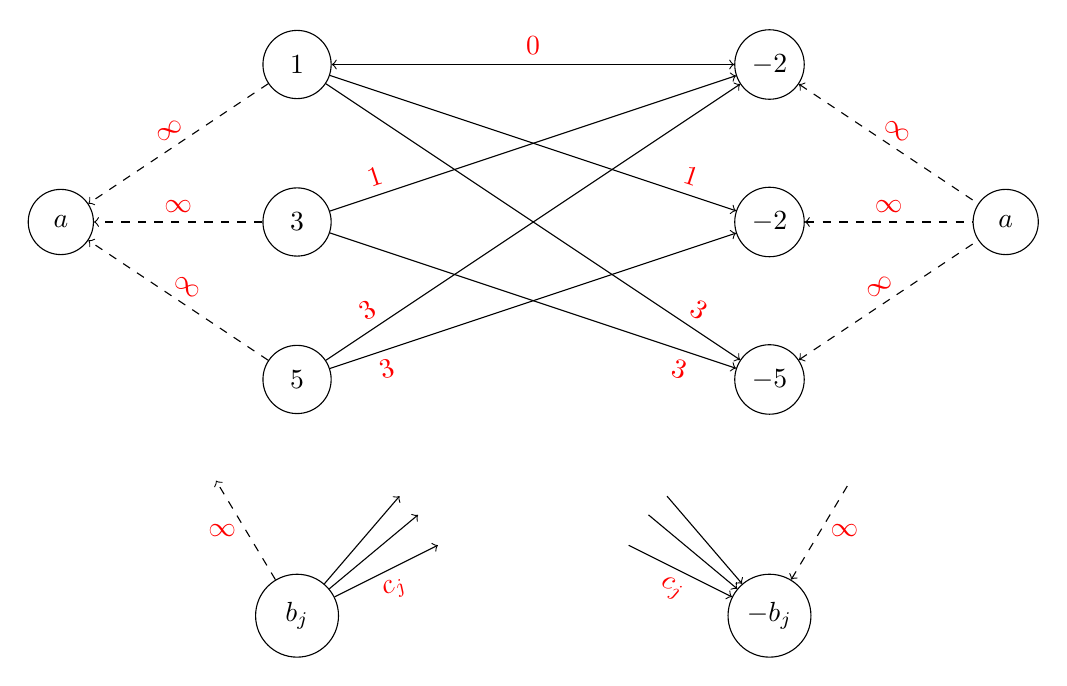
\begin{tikzpicture} [align=center]
\path (0, 4) node[circle, draw, text width=0.5cm] (v0) {$1$}
      (0, 2) node[circle, draw, text width=0.5cm] (v2) {$3$}
      (0, 0) node[circle, draw, text width=0.5cm] (v4) {$5$}
      (6, 4) node[circle, draw, text width=0.5cm] (v1) {$-2$}
      (6, 2) node[circle, draw, text width=0.5cm] (v3) {$-2$}
      (6, 0) node[circle, draw, text width=0.5cm] (v5) {$-5$}
      
      (-3, 2) node[circle, draw, text width=0.5cm] (al) {$a$}
      (9, 2) node[circle, draw, text width=0.5cm] (ar) {$a$}
      
      (0,-3) node[circle, draw, text width=0.65cm] (j0) {$b_j$}
      (6,-3) node[circle, draw, text width=0.65cm] (j1) {$-b_j$};
      
\draw[<->] (v0) to node [above, red] {$0$} (v1);
\draw[->] (v0) to node [sloped, anchor=center, above, red, very near end] {$1$} (v3);
\draw[->] (v0) to node [sloped, anchor=center, above, red, very near end] {$3$} (v5);
\draw[->] (v2) to node [sloped, anchor=center, above, red, very near start] {$1$} (v1);
\draw[->] (v2) to node [sloped, anchor=center, below, red, very near end] {$3$} (v5);
\draw[->] (v4) to node [sloped, anchor=center, above, red, very near start] {$3$} (v1);
\draw[->] (v4) to node [sloped, anchor=center, below, red, very near start] {$3$} (v3);

\draw[dashed, ->] (v0) to node [sloped, anchor=center, above, red] {$\infty$} (al);
\draw[dashed, ->] (v2) to node [above, red] {$\infty$} (al);
\draw[dashed, ->] (v4) to node [sloped, anchor=center, above, red] {$\infty$} (al);

\draw[dashed, <-] (v1) to node [sloped, anchor=center, above, red] {$\infty$} (ar);
\draw[dashed, <-] (v3) to node [above, red] {$\infty$} (ar);
\draw[dashed, <-] (v5) to node [sloped, anchor=center, above, red] {$\infty$} (ar);

\draw[->] (j0) to ($(j0)!2cm!(v1)$);
\draw[->] (j0) to ($(j0)!2cm!(v3)$);
\draw[->] (j0) to node [sloped, anchor=center, below, red] {$c_j$} ($(j0)!2cm!(v5)$);
\draw[dashed, ->] (j0) to node [left, red] {$\infty$} ($(j0)!2cm!(al)$);

\draw[<-] (j1) to ($(j1)!2cm!(v0)$);
\draw[<-] (j1) to ($(j1)!2cm!(v2)$);
\draw[<-] (j1) to node [sloped, anchor=center, below, red] {$c_j$} ($(j1)!2cm!(v4)$);
\draw[dashed, <-] (j1) to node [right, red] {$\infty$} ($(j1)!2cm!(ar)$);

\end{tikzpicture}
\end{document}